%--- Kapitel 3
\cleardoublepage
\chapter{Modelle im Softwareengineering}
\label{sec:Kap-3}

Warum beschäftigen wir uns im Rahmen einer Softwareengineering-Lehr\-ver\-an\-stal\-tung mit Modellen, wenn das Anliegen der Softwareentwicklung die Erstellung von funktionierendem Programmcode ist? Mal abgesehen davon, dass auch Programmcode ein Modell ist, nämlich das Modell des ausführbaren Programms – zunächst ein pragmatischer Grund: 
\marginline{der Sinn von Modellen}
An einem Softwareentwicklungsprojekt sind sehr viele unterschiedliche Personen und Personengruppen beteiligt, von denen die meisten in der Regel nicht programmieren können. Diskussionen oder Dokumentationen auf der Grundlage von Programmcode sind daher problematisch. Es braucht andere Formen für die Kommunikation und Zusammenarbeit der heterogenen Beteiligten, und im Softwareengineering – wie in vielen anderen Bereichen – sind das Modelle. Ein weiterer Grund ist die Mächtigkeit von Modellen: mit Modellen kann man frei wählbare Perspektiven auf das existierende oder zu erstellende Original (\zb das Softwareprodukt, die Realwelt oder den Softwareentwicklungsprozess) gestalten und damit auch die Komplexität der Softwareentwicklung reduzieren, indem man ganz gezielt nur einen bestimmten Aspekt oder eine bestimmte Blickrichtung berücksichtigt und alles andere zunächst ignoriert.



%--- Kapitel 3.1
\clearpage
\section{Der Modellbegriff}
\label{sec:Kap-3.1}

\vspace{-2mm} %%% für Druck

Der Begriff Modell ist in verschiedenen Disziplinen und Kontexten mit unterschiedlichen Bedeutungen belegt. Die wissenschaftlichen Modellbegriffe gehen aber alle mehr oder weniger stark auf die Arbeiten von Herbert Stachowiak zurück, der 1973 die „Allgemeine Modelltheorie“ \cite{sta73} veröffentlichte. Nach Stachowiak sind Modelle „Abbildungen [oder] Repräsentationen natürlicher oder künstlicher Originale, die selbst wieder Modelle sein können“ \cite[131]{sta73}. Über dieses sogenannte \textit{\mbox{Abbildungsmerkmal}} hinaus zeichnen sich Modelle nach Stachowiak dadurch aus, dass sie für einen spezifischen Adressaten(kreis) bestimmt sind, innerhalb bestimmter Zeit\-inter\-valle gültig sind und einen spezifischen Zweck verfolgen (\textit{Pragmatisches Merkmal}). Zudem erfassen Modelle nicht alle Merkmale ihres Originals, sondern nur diejenigen, die dem Ersteller des Modells für den Modellierungszweck relevant erscheinen (\textit{Verkürzungsmerkmal}). 

Ein Modell ist immer eine Abstraktion 
\marginline{Abstraktion}
des Originals. Das Original kann dabei bereits existieren, oder es soll noch erstellt werden. In der Softwareentwicklung ist meist Letzteres der Fall, ähnlich wie bei Modellen der Architektur (Hausbau, Brückenbau etc.). Abstraktion bedeutet, dass das Modell \textbf{keine vollständige} Darstellung des Originals ist. Zum einen wird es nur diejenigen Aspekte des Originals beinhalten, die dem Ersteller des Modells für den vorgesehenen Einsatz des Modells zweckmäßig erschienen. Zum anderen beinhaltet Abstraktion die Möglichkeit, dass Eigenschaften des Originals in einem geringeren Detaillierungsgrad als im Original dargestellt werden können. So könnte ein Modell eines Softwareprodukts zum Beispiel auf einer hohen Abstraktionsebene nur die großen Komponenten darstellen. Auf einer niedrigeren Abstraktionsebene könnte ein anderes Modell desselben Softwareprodukts jedes einzelne Softwareobjekt zeigen. Die Wahl einer geeigneten Abstraktionsebene für ein Modell ist neben den Punkten Einsatzzweck und Zielgruppe ein entscheidender Faktor für die Nützlichkeit des Modells. In diesem Zusammenhang sei erwähnt, dass im Softwareengineering ein konkretes Modell in der Regel nicht richtig oder falsch ist – wie es in Disziplinen oder Bereichen sein kann, in denen der Modell\-begriff stark mit dem Begriff der Theorie verknüpft ist. Es ist nur für die anvisierte Zielgruppe und den Einsatzzweck mehr oder weniger nützlich.

Im Softwareengineering werden Modelle in unterschiedlichen Situationen eingesetzt. Abbildung~\ref{fig:modellbegriff_softwareengineering} zeigt unter Rückgriff auf Stachowiaks allgemeinen Modellbegriff einen Modellbegriff für das Softwareengineering und seine verschiedenen Ebenen.

% Die Grafik ist breiter als die Textbreite.
\begin{figure}[t]
	\begin{addmargin*}[0cm]{-\marginparwidth}
	\begin{addmargin*}[0cm]{-\marginparsep}
		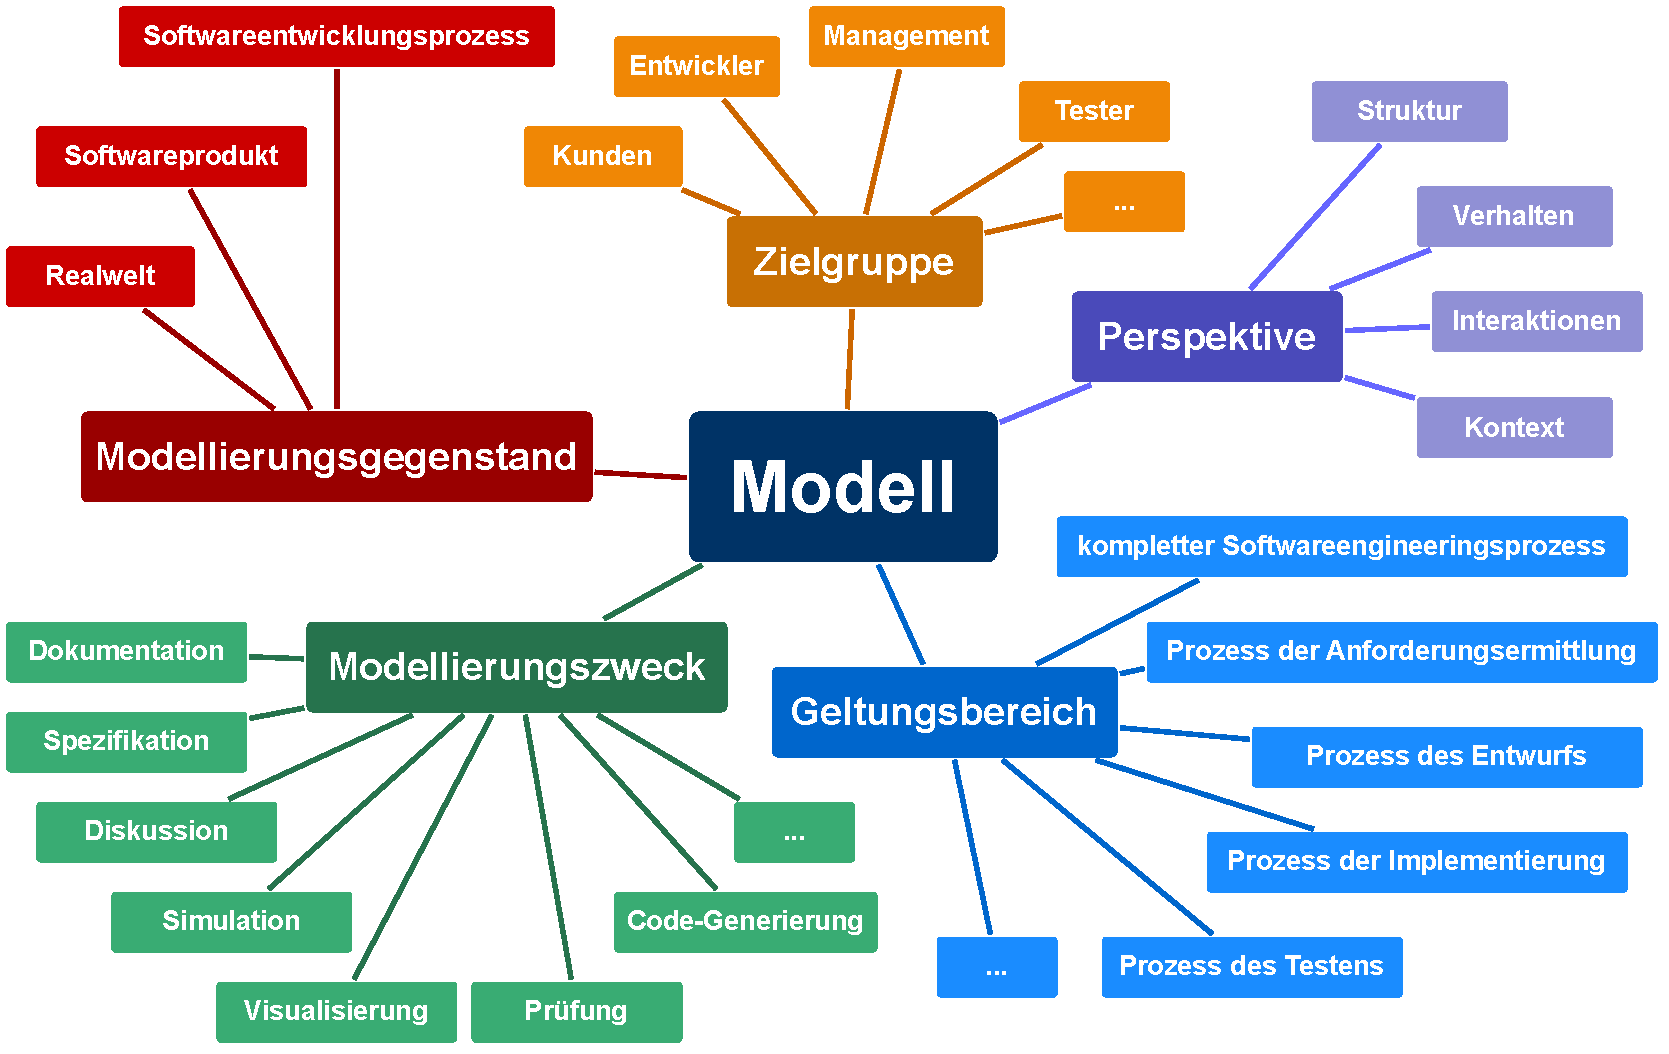
\includegraphics[scale=0.62]{Bilder/Kapitel-3/Abb-3-1-MindMap.pdf}
		\caption{Modellbegriff fürs Softwareengineering}
		\label{fig:modellbegriff_softwareengineering}
	\end{addmargin*}
	\end{addmargin*}
\end{figure}		

\vspace{1mm} % Ausgleich für den farblichen Kasten

\sttpMindMapText[colMindMap1]{\textbf{\textsf{Modellierungsgegenstand}}}
von Modellen können Softwareentwicklungsprozesse sein. Vertreter solcher Modelle haben Sie in Kapitel 2 %~\ref{sec:Kap-2}
mit den Vorgehensmodellen schon kennengelernt. Anstelle des Entwicklungsprozesses kann der Modellierungs\-gegenstand aber auch ein (zu entwickelndes) Softwareprodukt sein. In dieser Lektion werden Sie erstmalig Modelle kennenlernen, mit denen die \textbf{Realwelt} – bzw. genauer: der für die Entwicklung des Softwareprodukts relevante Ausschnitt der Realwelt, die sogenannte Domäne – abgebildet werden kann.

Eine weitere Ebene eines Softwareengineering-Modells ist die vom Modell eingenommene
\sttpMindMapText[colMindMap2]{\textbf{\textsf{Perspektive}}}
auf den Modellierungsgegenstand. Ein Modell kann die Struktur (\zb Aufbau, Elemente, statische Beziehungen zwischen Elementen) des Model\-lie\-rungs\-gegen\-stands zeigen, aber auch sein Verhalten (\zb Antwortverhalten auf \mbox{Ereignisse}) oder seine Interaktionen (zwischen verschiedenen Komponenten oder mit der Umgebung). Oder der Blickwinkel eines Modells ist auf die Abgrenzung zwischen dem Modellierungsgegenstand und seiner Umgebung gerichtet (die Perspektive Kontext in der Abbildung). Die aus Kapitel 2 %~\ref{sec:Kap-2}
bekannten Vorgehensmodelle betrachten in erster Linie die Struktur von Softwareentwicklungsprozessen und die Interaktion zwischen deren Komponenten, also den einzelnen Prozessen des Softwareengineering. 

\vspace{1mm} % Ausgleich für den farblichen Kasten

Der 
\sttpMindMapText[colMindMap3]{\textbf{\textsf{Geltungsbereich}}}
eines Vorgehensmodells ist meistens der komplette Softwareentwicklungsprozess. Andere Modelle im Softwareengineering, deren Modellierungsgegenstände ebenfalls Softwareentwicklungsprozesse sind, fokussieren sich nur auf bestimmte Teile dieses Softwareentwicklungsprozesses, zum Beispiel wenn sie nur den Prozess der Anforderungsermittlung im Blick haben. Für solche Modelle wird in Abgrenzung zum Begriff Vorgehensmodell häufig der Begriff \textit{Methode} verwendet – wobei der Begriff Methode in diesem Kontext nicht mit dem Begriff der Methode aus dem Kontext der Programmierung verwechselt werden darf. Der Begriff Methode ist im Softwareengineering sehr weit gefasst: Darunter fallen Konzepte, Para\-digmen, Strategien, Verfahren, Richtlinien oder sonstige Arten von Anleitungen, deren Ziel eine systematische Entwicklung von Software ist. So kann man sowohl die strukturierte Programmierung aus Abschnitt~1.1 %~\ref{sec:Kap-1.1}
als auch die Erhebung von Anforderungen mit Hilfe von Anwendungsfällen als Methode bezeichnen. In der Literatur wird auch Extreme Programming manchmal als Methode anstatt als Vorgehensmodell bezeichnet. Die Grenze zwischen Vorgehensmodell und Methode ist nicht immer eindeutig zu ziehen, insbesondere wenn sich ein Ansatz auf mehrere Prozesse des Softwareengineering bezieht. Letztendlich ist die Abgrenzung aber auch nur insofern relevant, dass man sowohl im Kapitel zu Methoden als auch im Kapitel zu Vorgehensmodellen eines Softwareengineering-Buchs suchen sollte, wenn man einen bestimmten Ansatz recherchieren möchte.

Im Softwareengineering werden zu einem Modellierungsgegenstand in der Regel mehrere Modelle erstellt. Durch unterschiedlich gewählte Abstraktionsebenen und unter\-schied\-liche Blickwinkel können schrittweise gezielt bestimmte Aspekte des abzu\-bildenden oder zu erstellenden Originals (Produkt, Prozess, Realwelt) untersucht werden und dabei jeweils Anforderungen oder Probleme des Gesamtkomplexes ausgeblendet werden. Insofern helfen Modelle bei der Verringerung von Komplexität – ein auf den verschiedensten Ebenen ganz zentrales Thema in der Software\-entwicklung. 

Außerordentlich wichtig 
bei der Erstellung jedes Modells sind die
\sttpMindMapText[colMindMap4]{\textbf{\textsf{Zielgruppe}}}
des Modells und der 
\sttpMindMapText[colMindMap5]{\textbf{\textsf{Modellierungszweck}}}. Die Kombination beider Faktoren bestimmt die konkrete Ausgestaltung des Modells. So wird zum Beispiel ein vom Entwicklungsleiter erstelltes Modell zur Diskussion mit dem Kunden über das Verhalten eines geplanten Softwareinkrements anders aussehen als das von derselben Person erstellte Modell für die gleiche Diskussion mit seinem Entwicklungsteam. Ebenso wird sich das Modell für den Kunden, das zu Diskussionszwecken erstellt wurde, von dem Modell für denselben Kunden unterscheiden, das zur Dokumentation der getroffenen Entscheidungen erstellt wird. Neben den in der Abbildung aufgeführten Zielgruppen und Modellierungszwecken sind viele weitere Gruppen und Zwecke denkbar. 

\sttpDefinitionskasten{\sttpDefinitionskastenSkalierungsfaktor}{Modell im Softwareengineering}{Die Abstraktion eines Originals, die für eine bestimmte Zielgruppe geschaffen wurde, einen definierten Einsatzzweck besitzt und eine spezifische Perspektive auf das Original einnimmt. Der Geltungsbereich des Modells kann der komplette Softwareentwicklungsprozess sein oder Teile davon.} 

\minisec{Modelle darstellen}
\phantomsection
\label{sec:Kap-3.1:Modelle_darstellen}
Damit man überhaupt mit Modellen arbeiten kann (über sie diskutieren, sie als Doku\-men\-ta\-tion verwenden etc.), müssen sie in irgendeiner Weise sichtbar sein. Das bedeutet, man benötigt Darstellungsmittel für Modelle. Im Rahmen des Softwareengineering werden Modelle häufig in Form von grafischen Notationen (Diagrammen) aufgeschrieben. Eine Notation ist eine Sammlung von (textuellen oder grafischen) Zeichen und Symbolen, die bestimmte Gegenstände oder Konzepte repräsentieren. Im Softwareengineering wird weitgehend synonym zum Begriff der Notation der Begriff der
\marginline{Modellierungs\-sprache}
\textit{Modellierungs\-sprache} verwendet. Modellierungssprachen legen einen Satz von Regeln fest, der bestimmten Elementen, zum Beispiel Kästchen oder \mbox{Pfeilen} einer bestimmten Form innerhalb eines Diagramms, eine jeweilige Bedeutung zuweist. Diese grafischen Darstellungen können um textuelle Darstellungen – in Form von Prosa oder in von der Modellierungssprache vorgegebener, stärker formularhafter Form – ergänzt werden. Die in diesem Text thematisierte Unified Modeling Language ist eine überwiegend grafische Modellierungssprache, die für verschiedene Zwecke aber auch textuelle Ergänzungen zu den Diagrammen anbietet. 

Neben den grafischen Modellierungssprachen werden im Softwareengineering auch rein textuelle Modellierungssprachen sowie formal-mathematische Notationen eingesetzt – allerdings deutlich seltener. Eine formalere Darstellung von Modellen anstelle der Diagrammdarstellung ist vor allem zu zwei Einsatzzwecken notwendig: Wenn aus im Rahmen der Softwareentwicklung erstellten Modellen automatisiert verfeinerte Modelle oder sogar Programmcode des zukünftigen Softwareprodukts erzeugt werden sollen, reichen grafische Diagramme nicht aus. Der zweite Einsatzzweck ist die formale Spezifikation – und damit auch mögliche formale Prüfung – von Anforderungen im Rahmen der Anforderungsermittlung und -analyse. 

Modelle im objektorientierten Softwareengineering setzen sich oft aus Submodellen zusammen. Jedes Submodell erfüllt seinen eigenen Zweck, indem es einen anderen Teil des Originals betrachtet oder einen anderen Blickwinkel einnimmt als ein anderes Submodell. Der  Begriff Modell 
\marginline{Modell und Diagramm}
und insbesondere die Abgrenzung zwischen den Begriffen Modell, Submodell und Diagramm wird in der Literatur uneinheitlich gehandhabt. Wir verfahren in diesem Kontext pragmatisch: Zum einen ist für uns ein Submodell gleichwertig mit einem Modell. So sind ein Strukturmodell und ein Verhaltensmodell zum selben Original einfach zwei Modelle, unabhängig davon, ob sie zusammen eingesetzt werden – und damit im strengen Sinne zwei Submodelle eines Gesamtmodells bilden würden – oder unabhängig voneinander das Original aus dem jeweiligen spezifischen Blickwinkel beschreiben.  Zum anderen gilt für die Beziehung zwischen Modell und Diagramm: Ein Diagramm (inklusive eventueller textueller Ergänzungen) bzw. eine Kombination aus mehreren Diagrammen \textbf{ist} die Manifestation eines Modells. Insofern wird in diesem Text beides als gleichbedeutend betrachtet. Wenn ein Diagramm verändert wird (\zb Elemente ergänzt oder Aspekte verfeinert) oder eine Menge zusammengehöriger Diagramme um ein weiteres Diagramm erweitert wird, entsteht ein neues Modell. 


%--- Kapitel 3.2
\clearpage
\section{objektorientierte Modellierung}
\label{sec:Kap-3.2}

Die  Bezeichnung objektorientierte Modellierung ist ein Sammelbegriff für den Einsatz objektorientierter Konzepte in den Software\-engineering-Prozessen Anforde-
\linebreak %%% für Druck
rungsermittlung und -analyse und Entwurf. Diese entstanden verstärkt seit Ende der 1980er und Anfang der 1990er Jahre. Oft findet sich in der Literatur auch die Aufteilung in die Begriffe \textit{objektorientierte Analyse} (engl. object oriented analysis, 
\marginline{OOA, OOD} 
OOA) und \textit{objektorientierter Entwurf} (engl. object oriented design, OOD). OOA und OOD sind dabei selbst wieder Oberbegriffe, unter denen eine Vielzahl konkreter und unterschiedlicher Methoden für das objektorientierte Softwareengineering subsumiert werden. Dementsprechend unterschiedlich werden OOA und OOD in der Literatur teilweise dargestellt. Gemeinsam ist den unterschiedlichen Methoden, dass für die Modellierungszwecke im Rahmen der Anforderungsermittlung und -analyse und derjenigen im Rahmen des Entwurfs dieselbe Notation – überwiegend die UML – verwendet wird. Beachten Sie, dass je nach verwendetem Vorgehensmodell für ein Softwareprojekt die Modellierung einen unterschiedlich großen Anteil einnimmt. So haben zum Beispiel sequentielle und agile Vorgehensmodelle durchaus verschiedene Vorstellungen über Umfang und Ausgestaltung der benötigten Modelle während des Softwareentwicklungsprozesses.

In dieser Lektion betrachten wir aus dem Themenbereich der objektorientierten Modellierung zunächst nur die Modellierung von Realweltzusammenhängen. 


\subsection{Objektorientierung}
\label{sec:Kap-3.2.1}

Die objektorientierte \textbf{Modellierung} hat ihren Ursprung in den Konzepten und Prinzipien der objektorientierten \textbf{Programmierung}. Die erste objektorientierte Programmiersprache war Simula67, die Ole-Johan Dahl und Kristen Nygaard in den 1960er Jahren entwickelten. Aus Simula67 stammt das für die Objektorientierung zentrale Grundkonzept von Klassen und Objekten. Die seit den 1970er Jahren von Adele Goldberg, Dan Ingalls und  Alan Kay entwickelte Programmiersprache Smalltalk \cite{gol83} ist damit zwar nicht die erste objektorientierte Programmiersprache; sie gilt trotzdem heute als Ursprung der Objektorientierung, da sie in Simula67 angelegte Konzepte, wie Datenkapselung und Vererbung, konsequent objektorientiert aus\-arbeitete und um neue Konzepte wie Polymorphie und dynamisches Binden ergänzte, die heute zu den zentralen Charakteristika der Objektorientierung zählen. Seit Ende der 1980er Jahre lösten objektorientierte Programmiersprachen zunehmend andere Arten von Programmiersprachen (wie die strukturierte Programmierung) ab. 

Die 
\marginline{Ziele}
objektorientierte Programmierung erhob den Anspruch, die Komplexität von Softwareentwicklung reduzieren zu können, Software besser testbar, besser wartbar und einfacher erweiterbar zu machen und die Wiederverwendung von Konzepten und Programmcode zu fördern. Dazu beinhaltete sie verschiedene (Entwurfs)Prinzipien wie Datenkapselung, Geheimnisprinzip, Modularisierung, Vererbung, Polymorphie und Abstraktion. Die heute verbreiteten objektorientierten Programmiersprachen weichen von der durch Smalltalk begründeten reinen Lehre der Objektorientierung allerdings in einigen Aspekten ab (\zb primitive Datentypen). Zudem zwingen sie die Programmierer unterschiedlich strikt zur Einhaltung dieser objektorientierten Prinzipien. Das hat zur Folge, dass es auch mit objektorientierten Programmiersprachen durchaus möglich ist, nicht-objektorientiert zu implementieren. 

Die  Basis der Objektorientierung ist das \textit{Objekt}.
\marginline{Objekt}
Ein Objekt in einer Software ist eine Einheit aus Daten und Operationen, die auf diesen Daten arbeiten. Damit unterscheidet sich die Objektorientierung von der zuvor verbreiteten strukturierten Programmierung, wie sie zum Beispiel mit Programmiersprachen wie Pascal und C verbunden ist. In der strukturierten Programmierung werden Daten und Operationen als getrennte Einheiten behandelt. Die Programmierer der Software müssen darauf achten, dass die Operationen auf den richtigen Daten arbeiten. Nach der reinen objektorientierten Lehre dagegen arbeiten auf den Daten eines Objekts nur seine eigenen Operationen. 

Zur Laufzeit der Software existiert eine (durch den Programmcode definierte) veränderliche Menge von Software-Objekten, die in Beziehungen zueinander stehen und miteinander interagieren.

Neben  der Kapselung von Daten und Operationen in einem Objekt besteht die zentrale Idee der Objektorientierung in der engen Orientierung an der Realwelt. 
\marginline{Realweltbezug – das zentrale Konzept der Objekt\-orientierung}
Die Objektorientierung versucht Strukturen der Realwelt in Software nachzubilden. Dafür werden die Objekte der Software anhand der Merkmale und des Verhaltens von Objekten des zu modellierenden Realweltausschnitts (Domäne) konstruiert. Dabei ist es wichtig, geeignete Abstraktionsebenen zu wählen: Für die Konstruktion der Software-Objekte werden nur diejenigen Merkmale der Realwelt-Objekte berücksichtigt, die für den Anwendungszweck des zukünftigen Softwareprodukts relevant sind. 

\begin{figure}[h!]
	\centering
	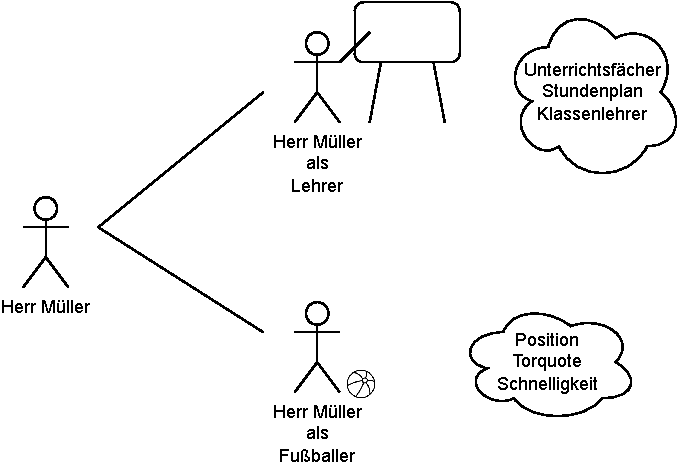
\includegraphics{Bilder/Kapitel-3/mueller_lehrer_fussballer.pdf}
	\caption{Herr Müller als Lehrer und als Fußballer}
	\label{fig:mueller_lehrer_fussballer}
\end{figure}

Abbildung~\ref{fig:mueller_lehrer_fussballer} zeigt 
\marginline{das Prinzip der Abstraktion}
links die Realwelt-Person Herrn Müller – bzw. ein Strichmännchen, von dem wir so tun, als sei es Herr Müller. Herr Müller ist von Beruf Lehrer und in seiner Freizeit begeisterter Fußballer. Angenommen, wir möchten eine Schul\-verwal\-tungs\-soft\-ware entwickeln, in der der Realwelt-Lehrer Herr Müller als Software-Objekt Lehrer Müller vorkommen soll. In diesem Fall würden uns Merkmale des Realwelt-Menschen Herrn Müller interessieren, die mit seinem Lehrerberuf zu tun haben, zum Beispiel welche Fächer unterrichtet er, wie sieht sein Stundenplan aus, ist er Klassenlehrer? Wenn wir statt einer Schulverwaltungssoftware ein Wettportal für Fußballwetten entwickeln wollten, würde uns an Herrn Müller dagegen interessieren, auf welcher Position er spielt, welche Torquote er hat und wie hoch seine Schnelligkeit ist. 

Bei der Konstruktion von Software-Objekten geht es darum, die für die zu erstellende Software relevanten Charakteristika von Realwelt-Objekten abzubilden und von allen anderen Merkmalen der Realwelt-Objekte zu abstrahieren. Wie das konkret geht, sehen wir uns in Kapitel~\ref{sec:Kap-4} an. Zunächst beschäftigt uns hier das Domänenmodell -- das alle diese modellierten Realwelt-Objekte später umfasst -- nochmal als Ganzes.
\subsection{Das Domänenmodell}
\label{sec:Kap-3.2.2}

Wie aus der Darstellung des Modellbegriffs in Abschnitt~\ref{sec:Kap-3.1} bekannt, kann man Modellierung im Softwareengineering in sehr unterschiedlichen Kontexten einsetzen. Für die Vorbereitung der konkreten Implementierung könnte man zum Beispiel ein Modell erstellen, das sehr technisch gehalten ist und genau diejenigen Elemente enthält, die in der ausgewählten Programmiersprache implementiert werden sollen. Am anderen Ende der Skala kann Modellierung auch verwendet werden, um Strukturen und Abläufe der Realwelt zu modellieren, ohne Implementierungsbedürfnisse zu berücksichtigen. Im objektorientierten Softwareengineering nennt man letzteres Modell ein Domänenmodell. 

Der Begriff der \textit{Domäne} \marginline{Domäne}
wird in unterschiedlichen Wissensgebieten äußerst unterschiedlich definiert. Im Softwareengineering ist eine Domäne derjenige Ausschnitt der Realwelt, der (entsprechend abstrahiert) in der zukünftigen Software abgebildet werden soll. Die Domäne umfasst also Objekte, Strukturen, Arbeits-, Geschäfts\-prozesse und sonstige Abläufe, Personengruppen, Interaktionen, Beziehungen etc. eines abgegrenzten Bereichs der Realwelt. Zum Beispiel würde für eine zu erstellende Schulverwaltungssoftware die Domäne Schule, für ein Fußball-Wettportal die Domäne Fußball relevant sein. Anstelle des Begriffs Domäne wird manchmal auch von Fachgebiet, Anwendungsbereich oder fachlichem Problembereich gesprochen. Ein \textit{Domänenmodell}
\marginline{Domänen-\\modell}
(engl. domain model) – in englischsprachiger Literatur teilweise auch semantic (information) model oder conceptual (information) model – beschreibt entsprechend (Abstraktionen der) Objekte, Strukturen und Abläufe der Domäne und zwar in den Begrifflichkeiten der Domäne, sodass das Domänenmodell auch von Personen außerhalb des Softwareentwicklungsteams verstanden werden kann. In der objektorientierten Softwareentwicklung werden zur Erstellung von Domänenmodellen häufig die Diagrammtypen der Unified Modeling Language (UML) verwendet.

In der Regel besteht ein Domänenmodell sowohl aus statischen (Objekte, Beziehungen, Strukturen) als auch aus dynamischen (bestehende bzw. zu gestaltende Pro\-zesse, Abläufe und Interaktionen) Perspektiven, sogenannten \textit{Sichten},
\marginline{Sicht}
auf die \mbox{Domäne.} Dafür werden meist unterschiedliche Arten von Diagrammen sowie informelle textuelle Beschreibungen kombiniert. Bei  Einsatz von UML als Modellierungssprache ist das Kernstück des Domänenmodells das \textit{Domänenklassendiagramm}, das eine statische Sicht auf die Domäne liefert. Darüber hinaus umfasst ein Domänenmodell häufig verschiedene Arten grafischer oder textueller Beschreibungen, zum Beispiel zur Struktur von Organisationseinheiten (statische Sicht), zur Interaktion zwischen Elementen der Domäne (dynamische Sicht) oder zu Geschäftsprozessen der Domäne (dynamische Sicht).

\vspace{2.2mm} %%% für Druck

\minisec{Anforderungsermittlung und Domänenmodell}
\phantomsection
\label{sec:Kap-3.2-2:anforderungsermittlung}

\vspace{1.1mm} %%% für Druck

Mit der Erstellung eines Domänenmodells wird parallel zu der Anforderungsermittlung begonnen. Oft lassen sich Tätigkeiten nicht eindeutig der Anforderungsermittlung oder der Domänenmodellerstellung zuordnen. So können zum Beispiel modellierte Geschäftsprozesse sowohl Auskunft über Arbeitsabläufe der Domäne geben als auch direkte Anforderungen sein, wenn das zu entwickelnde Softwareprodukt genau diese Geschäftsprozesse unterstützen soll. In Softwareentwicklungsprojekten, die nach sequentiell orientierten Vorgehensmodellen arbeiten, wird das Domänenmodell innerhalb der Phase der Anforderungsermittlung und -analyse abgeschlossen, in agilen Softwareentwicklungsprojekten unterliegt das Domänenmodell – sei es implizit oder explizit vorhanden – genau wie die Anforderungen kontinuierlichen Veränderungen während der gesamten Entwicklungszeit des Softwareprodukts. 

Das Domänenmodell wird vom Softwareentwicklungsteam erstellt, unter enger Einbindung von Personen, die sich mit der Domäne auskennen (Domänenexperten).
In der Regel kommen die Domänenexperten aus dem Umfeld des Auftraggebers des Softwareprodukts (\zb Mitarbeiter verschiedener Fachabteilungen). \marginline{Ziel} Hauptzweck eines Domänenmodells ist die Schaffung eines gemeinsamen (Begriffs)Verständnisses von Softwareentwicklungsteam und Kunde über die Domäne. Adressat des Domänenmodells ist zum einen der Kunde. Dieser muss kontrollieren können, ob das entstandene Modell die Domäne adäquat abbildet. Dementsprechend nicht-technisch muss das Domänenmodell gestaltet sein. Aber auch das Entwicklungsteam (bzw. zumindest einzelne Personen des Teams) ist Zielgruppe des Domänenmodells. Dies ist ein Aspekt, der in Softwareentwicklungsprojekten leider oft vernachlässigt wird. Vom Kunden kann nicht erwartet werden, im weiteren Verlauf des Softwareentwicklungsprozesses (technische) Entwurfsentscheidungen der Software oder gar fertigen Programmcode daraufhin zu überprüfen, ob die Gegebenheiten der Domäne berücksichtigt worden sind. Das ist Aufgabe des Entwicklungsteams und dieses muss dafür die Domäne verstanden haben. 

In klassisch organisierten Softwareentwicklungsprojekten gibt es häufig die Rolle \textit{\mbox{Requirement} Engineer}. 
\marginline{Requirement Engineer}
Diese bildet das Bindeglied zwischen Kunde und Entwicklungsteam. Der Requirement Engineer hat die Aufgabe, die Anforderungen des Kunden und in diesem Zusammenhang auch dessen Wissen über die Domäne zu verstehen und sie für die Softwareentwickler im Team so aufzubereiten, dass diese das Softwareprodukt erstellen können, ohne sich in allen Einzelheiten mit der Domäne auseinandergesetzt zu haben. In agilen Projekten, in denen es in der Regel weniger feste Rollenzuordnungen innerhalb des Teams gibt, ist die Verfügbarkeit des notwendigen Domänenwissens bei den Softwareentwicklern schwieriger sicherzustellen. 

Die finale Version des Domänenmodells enthält genau die Aspekte der Realwelt, die eine Relevanz für das zukünftige Softwareprodukt haben. Die Erstellung eines Domänenmodells ist ein (in der Regel sehr kommunikationsintensiver) Prozess. Es erfordert viel Abstimmung zwischen Kunde und Entwicklungsteam und oft mehrere Modell-Zwischen\-ver\-sionen bis ein Domänenmodell fertiggestellt ist. In vielen Softwareentwicklungsprojekten spielt dabei auch eine Rolle, dass zu Beginn zunächst die Systemgrenzen des zukünftigen Softwareprodukts abgestimmt bzw. verhandelt werden müssen und in diesem Zusammenhang auch erstmal noch unklar sein kann, welcher Ausschnitt der Realwelt denn die Domäne bildet.

Zum Schluss sei noch darauf hingewiesen, dass eine Domäne nicht unveränderlich ist. Zum einen können sich Strukturen oder Abläufe (\zb Arbeitsprozesse) während der Erstellungszeit des Softwareprodukts ändern. Zum anderen könnte es gewünscht sein, Arbeitsprozesse etc. einer Domäne zu verändern, sobald das Softwareprodukt zur Verfügung steht, das diese Arbeitsprozesse übernehmen oder unterstützen kann. In diesem Fall ist die Domäne, die im Rahmen der Erstellung des Softwareprodukts modelliert wird, nicht die aktuell existierende, sondern die zukünftige Domäne. Beispiel: In der Beschreibung ihres Zoos (s. Lektion 1, Fallbeispiel Zoo) spricht die Zoodirektorin davon, dass aktuell sowohl Gehege als auch Käfige für die Tiere verwendet würden, dass es zukünftig aber ausschließlich Gehege geben solle. Bei der Domänenmodellierung wäre in diesem Beispiel daher zu klären, inwiefern die Käfige überhaupt berücksichtigt werden sollen.
\subsection{Die Unified Modeling Language (UML)}
\label{sec:Kap-3.2.3}

Der zentrale Faktor für die Qualität von Modellen, die im Rahmen des Softwareentwicklungsprozesses erstellt werden, ist ihre Eignung für die anvisierte Zielgruppe und den vorgesehenen Einsatzweck. Das bedeutet, dass die Menschen, die das Modell verstehen sollen, es auch verstehen können müssen und anhand des Modells die Entscheidungen treffen können, die sie treffen sollen. Dies kann aber nur gelingen, wenn die eingesetzte Modellierungssprache zum einen eindeutig genug ist, um Missverständnisse zu vermeiden und zum anderen mächtig genug ist, um alle benötigten Konzepte abbilden zu können. Idealerweise sollte sie zudem für die gegebenenfalls auch aus technisch nicht-versierten Personen bestehende Zielgruppe leicht erlernbar sein. Eine wichtige Aufgabe zu Beginn eines Softwareentwicklungsprojekts ist daher die Verständigung auf die einzusetzende(n) Modellierungssprache(n). Eine in vielen objektorientierten Softwareentwicklungsprojekten eingesetzte Modellierungssprache ist die Unified Modeling Language (UML). Die UML ist eine sehr mächtige Modellierungssprache, die die gängigen Konzepte der Objekt\-orien\-tierung abbilden kann. Gleichzeitig bietet sie sehr unterschiedliche Diagrammtypen an, mit denen sich verschiedene Sichten auf die Domäne oder das bestehende bzw. zu entwickelnde Softwareprodukt modellieren lassen. 

In den späten 1980er und frühen 1990er Jahren waren von unterschiedlichen Autorinnen und Autoren verschiedene Methoden und zugehörige Notationen für objekt\-orientiertes Softwareengineering vorgestellt worden. Zu den bekannteren gehörten die Object Modeling Technique (OMT) von James Rumbaugh  \cite{rum91}, die Booch-Methode von Grady Booch \cite{boo94} und das Object-Oriented Software Engineering (OOSE) von Ivar Jacobsen \cite{jac92}. Mitte der 1990er Jahre führten Booch, Jacobson und Rumbaugh – zu diesem Zeitpunkt mittlerweile alle drei bei Rational Software beschäftigt – ihre Ansätze zusammen, integrierten Notationen weiterer Autorinnen und Autoren und schufen mit der UML eine einheitliche Modellierungssprache für die objektorientierte Softwareentwicklung. 

Die Version 1.0 der UML wurde 1997 veröffentlicht. Die UML verbreitete sich \mbox{rasant}, auch weil sie seit Ende der 1990er Jahre als Standard der Object Management Group  (OMG), in der zahlreiche Unternehmen der Computerindustrie vertreten sind, herausgegeben wird und seitdem unter Führung der OMG kontinuierlich weiterent\-wickelt wird. 

Die UML definiert (in erster Linie grafische) Symbole, mit denen objektorientierte Konzepte (wie \zb Objekt, Klasse, Schnittstelle, Generalisierung, Nachrichten\-versand) dargestellt werden können. Die grafischen Notationselemente sind bewusst sehr einfach gehalten, um UML-Diagramme auch für Nicht-Programmierer verständlich zu gestalten. Vereinfacht gesagt, bestehen UML-Diagramme fast ausschließlich aus Kästchen und Pfeilen zwischen den Kästchen. 

Mit dem Wechsel auf Version 2.0 im Jahr 2005 wurde die UML komplett neu strukturiert. Ein Ziel war es, die UML allgemeingültiger objektorientiert zu halten, indem Notationselemente noch unabhängiger von den Bedürfnissen konkreter objektorientierter Programmiersprachen gestaltet wurden. Außerdem erweiterte die Version 2 die UML um zusätzliche Diagrammarten, vor allem um dynamisches Verhalten eines Softwaresystems noch besser modellieren zu können. Mit der Object Constraint Language 
(OCL) wurde zudem eine formale Beschreibungssprache in die UML integriert, mit der man grafische Notationselemente mit zusätzlichen Zusicherungen und Bedingungen versehen kann. Die aktuelle Version der UML ist heute (2024) die Version 2.5.1, die im Dezember 2017 veröffentlicht wurde.\footnote{Die jeweils aktuelle UML-Spezifikation kann frei von der Website der OMG heruntergeladen werden: \url{https://www.omg.org/spec/UML/About-UML/}}

Die UML bietet sieben sogenannte Strukturdiagramme an, mit denen sich aus einer statischen Sicht Elemente (\zb Module, Klassen, Objekte) und ihre Beziehungen zueinander modellieren lassen. Hinzu kommen sieben sogenannte Verhaltens\-diagramme, mit denen aus einer dynamischen Sicht Prozessabläufe sowie Inter\-aktionen zwischen Elementen modelliert werden können.

Die UML ist eine reine Modellierungs\textbf{notation}, sie ist \textbf{keine Methode} für objekt\-orientiertes Softwareengineering. Das bedeutet, sie stellt verschiedene Diagrammtypen zur Verfügung und gibt vor, welche Notationselemente in welchen Diagrammen und in welchen Kombinationen verwendet werden können. Sie legt aber nicht fest, welche Diagramme, in welcher Detailtiefe und in welcher Reihenfolge für die Durchführung der Prozesse des Softwareengineering erstellt werden sollen. Daher besitzen die verschiedenen UML-Diagrammtypen auch explizit keine feste Zuordnung zu konkreten Tätigkeiten des Softwareengineering, sondern können für verschiedene Software\-engi\-neering-Prozesse verwendet werden. So eignen sich zum Beispiel UML-Klassen\-dia\-gramme in entsprechend angepassten Abstraktionsgraden sowohl für die Domänenmodellierung als auch für die Prozesse der Anforderungsermittlung und -analyse und des Entwurfs sowie für die Prozesse der (Vorbereitung der) Implementierung und des Testens. In dieser
\marginline{Durchgängigkeit der Konzept\-modellierung}
Durchgängigkeit der Konzeptmodellierung über verschiedene Prozesse des Softwareengineering liegt einer der großen Vorteile der UML. UML-Diagramme aus frühen Phasen der Softwareentwicklung können durch Ergänzungen und Verfeinerungen in geeignete Diagramme für spätere Phasen überführt werden. Medienbrüche können dabei weitgehend vermieden werden.

\sttpKasten{\textbf{UML-Werkzeuge}

Parallel zur Entwicklung und Weiterentwicklung der UML entstanden Werkzeuge zur Erstellung von UML-Diagrammen. Grundsätzlich lassen sich UML-Diagramme mit allen gängigen Zeichenprogrammen erstellen, mit denen man verschiedene Arten von Kästen und Pfeilen zeichnen kann. Explizite UML-Zeichenprogramme bieten aber den Vorteil, dass die verschiedenen UML-Notationselemente direkt ausgewählt werden können und dass die Programme bei der Einhaltung der Syntax-Regeln (welche Notationselemente dürfen in welchen Kombinationen verwendet werden) unterstützen. Seit der Version 2 der UML existiert mit dem XML Metadata Interchange-Format (XMI) zudem ein standardisiertes Austauschformat für die Speicherung von UML-Diagrammen. Sofern die UML-Werkzeuge dieses Format unterstützen, kann auf diese Weise ein UML-Diagramm, das mit einem bestimmten UML-Werkzeug erstellt wurde, auch mit einem anderen UML-Werkzeug angezeigt und weiter bearbeitet werden.

Neben den reinen UML-Zeichenprogrammen gibt es UML-Werkzeuge, die auf Grundlage eines im Entwurfsprozess erstellten UML-Klassendiagramms des zukünftigen Softwareprodukts Programmcode einer bestimmten objektorientierten Programmiersprache erzeugen. Diese Automatisierung des Implementierungsprozesses bietet – zumindest theoretisch – den Vorteil, dass Inkonsistenzen zwischen Entwurfsmodell und Programmcode verhindert werden können, indem Änderungen nur am Modell vorgenommen werden und der Programmcode \mbox{daraus} automatisiert erzeugt wird.}

Sie werden verschiedene Diagramme der UML kennenlernen, die in den Prozessen des Softwareengineering eingesetzt werden können. Es geht uns explizit nicht darum, im Rahmen dieses Textes die UML in ihrer Gänze darzustellen. Die Notationselemente der UML interessieren (nur) vor dem Hintergrund ihrer Einsatzmöglichkeiten für Aktivitäten im Softwareengineering und werden daher in Zusammenhang mit den – und begrenzt auf die – in der jeweiligen Lektion gerade behandelten Themen des Softwareengineering vorgestellt. 




\subsection{objektorientierte (Domänen)Modellierung und agile Ansätze}
\label{sec:Kap-3.2.4}

\sttpzitat{„I was astonished to be invited to what became the meeting that originated the Agile Manifesto because my work had always been based around building models.“ \cite[17]{hun11}}{}

So Stephen J. Mellor, einer der Autoren des Agilen Manifests, im Rückblick.

\pagebreak %%% für Druck

Modelle verbindet man im Allgemeinen tatsächlich eher nicht mit agiler Softwareentwicklung, da Letztere die Bereiche der Programmcodeerstellung und des Testens in den Vordergrund der Softwareentwicklung stellt, während man Modelle vor allem in den Prozessen der Anforderungsermittlung und -analyse sowie des Entwurfs antrifft. Zudem gehört es zur anvisierten Leichtgewichtigkeit der agilen Softwareentwicklung, dass außer dem Programmcode möglichst wenige Artefakte produziert werden (und konsistent gehalten werden müssen). Dagegen haben UML-Diagramme meistens zumindest  \textbf{auch} die Aufgabe, Aspekte zu dokumentieren und müssen daher kontinuierlich mit entsprechendem (Personal)Aufwand aktuell gehalten werden. Insofern passen UML-Modelle und agile Softwareentwicklung nicht unmittelbar zusammen. Mehrere zusammengehörige UML-Diagramme, mit denen verschiedene Sichten auf ein (zu entwickelndes) Softwareprodukt modelliert werden, findet man in agilen Softwareentwicklungsprojekten daher in der Regel kaum.

\textbf{Wenn} zukünftige Softwareprodukte Modellierungsgegenstand in agilen Software\-entwicklungsprojekten sind, dann überwiegend mit dem Fokus, im Entwicklungsteam oder mit dem Kunden über bestimmte Aspekte der Software zu diskutieren. Hier steht der Kommunikationszweck 
\marginline{Modelle für Kommunika\-tions\-zwecke}
und weniger der Spezifikationszweck als Grundlage der späteren Implementierung oder der Dokumentationszweck für getroffene Entscheidungen im Vordergrund. Entsprechend kann es sich bei den Modellen anstelle von UML-Diagrammen um einfache Skizzen am Whiteboard, Post-its, Bilder oder Prototypen von Benutzeroberflächen oder kurze textuelle Beschreibungen handeln, über die zudem eher mündlich als schriftlich kommuniziert wird. Die Modelle müssen daher meistens auch nicht für sich selbst sprechen, sondern sind (nur) Bestandteil von Kommunikationszusammenhängen. Scott  W. Ambler, 
\marginline{agiles Modellieren}
ein überzeugter Vertreter agilen Vorgehens, hat im Rahmen seines Ansatzes „Agile Modeling“ \cite{amb02} Prinzipien für ein leichtgewichtiges Modellieren aufgestellt. Danach müssen Modelle in der agilen Softwareentwicklung nicht umfassend sein, nicht in jeder Hinsicht konsistent sein und auch nicht für die gesamte Dauer des Entwicklungsprojekts gültig bleiben. Sie können sehr einfach gehalten sein und müssen nur in der konkreten Situation, in der bzw. für die sie modelliert werden, verständlich sein und ihren Einsatzzweck erfüllen.

\vspace{3mm} %%% für Druck

\sttpseitenrandzitat{„An agile model is a model that is just barely good enough.“ \cite[12]{amb02}}{Scott W. Ambler über agile Modelle}

\vspace{3mm} %%% für Druck

Im  Bereich der \textbf{Domänen}modellierung 
\marginline{agile Domänen\-modellierung}
unterscheiden sich klassische und agile Ansätze auch, aber weniger deutlich als bei der Modellierung von Softwareprodukten. Die Einbeziehung des Domänenwissens in den Softwareentwicklungsprozess – in der Regel über die Einbeziehung von Kunden und Domänenexperten – ist ein zentraler Bestandteil agiler Softwareentwicklung und findet in jeder Iteration statt. In jeder Iteration wird eine bestimmte Menge von Anforderungen bestimmt und in Programmcode umgesetzt. Diese Anforderungen stehen im Fokus. Tätigkeiten zur Modellierung der Domäne finden in der Regel insoweit statt, wie sie im Rahmen der zu erfüllenden Anforderungen benötigt werden. Modelliert werden diejenigen Objekte, Strukturen, Interaktionen etc. der Domäne, bei denen es einen Zusammenhang zu den aktuellen Anforderungen gibt. Das Domänenmodell entsteht so nicht ein einziges Mal als Ganzes wie in sequentiellen Ansätzen, sondern wächst mit jeder Iteration an. Damit ist es deutlich stärkeren Anpassungen im Laufe des Projekts ausgesetzt als in sequentiell orientierten Projekten.

Es hängt sehr vom konkreten agilen Projekt ab, inwiefern das Domänenwissen \textbf{\mbox{explizit}} dokumentiert wird (zum Beispiel über ein UML-Domänen\-klassen\-diagramm, die Erstellung eines Glossars, die grafische oder textuelle Darstellung von Geschäfts\-prozessen etc.) oder implizit bleibt, zum Beispiel weil Domänenexperten täglich für Fragen des Entwicklungsteams persönlich zur Verfügung stehen können. 


%--- Kapitel 3.3 KommLit
\clearpage
\section{Kommentierte Literatur}
\label{sec:Kap-3.3}

\sttpKommLitItem{Stachowiak}{1973}{Allgemeine Modelltheorie}{sta73}{Bilder/Buchcover/Buchcover_Stachowiak.jpg}{}
{Eine sehr umfassende Auseinandersetzung mit vorher vorhandenen Erkenntnissen zum Bereich des Modells und darauf aufbauend die Entwicklung einer eigenen sehr ausdifferenzierten Modelltheorie. Diese hat sich heutzutage als Standard für wissenschaftliche Modellbegriffe etabliert. Für den Zweck dieses Kapitels benötigen wir nur die Grundlagen von Stachowiaks Modelltheorie, wie sie in Kapitel 2.1 des Buchs dargestellt werden.
}

\sttpKommLitItem{Balzert}{2005}{Lehrbuch der Objektmodellierung}{bal05}{Bilder/Buchcover/Buchcover_Balzert.jpg}{}
{Das Lehrbuch beschäftigt sich mit Methoden der objektorientierten Analyse (OOA) und des objektorientierten Entwurfs (OOD). In diesem Zusammenhang werden mit vielen Beispielen die Notationselemente der UML vorgestellt – jeweils in dem für OOA bzw. OOD benötigten Detaillierungsgrad. Kapitel 1 enthält zudem eine recht ausführliche Beschreibung der Entwicklungsgeschichte der UML.}

\sttpKommLitItem{Kecher/Salvanos/Hoffmann-Elbern}{2018}{UML 2.5}{kec18}{Bilder/Buchcover/Buchcover_Kecher_Salvanos.jpg}{}
{Die offizielle Spezifikation der UML, die frei von der Website der OMG heruntergeladen werden kann (\url{https://www.omg.org/spec/UML/About-UML/}), ist gerade für UML-Anfänger wenig übersichtlich. Sekundärliteratur zur UML ist daher sehr hilfreich. Dieses Buch bietet eine sehr gute und übersichtliche Darstellung der Diagrammarten und Elemente der UML 2.5 sowie eine kurze Übersicht zur Geschichte der UML. Es ist bereits die 6. Auflage des Buchs. Bisher ist mit jeder größeren Änderung der UML eine neue Auflage erschienen. Jede Diagrammart wird in einem eigenen Kapitel behandelt und nach ähnlichem Schema vorgestellt. Dazu gehören die Beschreibung der einzelnen Notationselemente anhand zahlreicher unterschiedlicher Lebensweltbeispiele genauso wie Beispiel-Implementierungen von in UML modellierten Konzepten in Java- und C\#-Programmcode. Zudem findet sich zu Beginn jedes Kapitels eine kurze Übersicht, zu welchen Zwecken das jeweilige Diagramm im Rahmen von Softwareengineering-Prozessen üblicherweise verwendet wird.}

\sttpKommLitItem{Bourque/Fairley (Hrsg.)}{2014}{SWEBOK V3.0 – Kapitel 9}{swe14}{Bilder/Buchcover/Buchcover_SWEBOK.jpg}{}
{Der schon bekannte Software Engineering Body of Knowledge (SWEBOK) behandelt in Kapitel 9 „Software Engineering Models and Methods“ auch das Thema Modelle im Softwareengineering. Die Konzepte Modell und Abstraktion werden beschrieben, verschiedene Modelltypen vorgestellt sowie über den Sinn von Modellierung und über Gütekriterien für Modellierungssprachen referiert. Wie in den anderen SWEBOK-Kapiteln ist der Stil sehr konzeptionell, teilweise abstrakt, gehalten. Als erster Einstieg in das Thema Modellierung ist der Artikel daher eher weniger geeignet, stattdessen aber sehr gut, wenn einem die Begrifflichkeiten des Themas bekannt, die Abgrenzungen zwischen einzelnen Konzepten aber etwas unklar geblieben sind.}

\sttpKommLitItem{Ambler}{2002}{Agile Modeling}{amb02}{Bilder/Buchcover/Buchcover_Ambler_02.jpg}{}
{Der Autor Scott W. Ambler ist ein starker Befürworter agiler Softwareentwicklung. Nichtsdestotrotz legt er großen Wert auf den Einsatz von Modellen im Rahmen von Softwareentwicklungsprojekten. In diesem Buch stellt er seine Methode eines agilen Modellierens vor, mit der agile Prinzipien und Tätigkeiten der Modellierung in Einklang gebracht werden sollen. Auf dieser Methode basiert auch Amblers spätere Veröffentlichung zum objektorientierten Modellieren. \cite{amb04}.}

\sttpKommLitItem{Ambler}{2004}{The Object Primer}{amb04}{Bilder/Buchcover/Buchcover_Ambler_04.jpg}{}
{Das Buch stellt vor, in welcher Weise objektorientierte Modellierungstechniken mit agilen Prinzipien verbunden werden können. In Kapitel 8 des Buches werden
	\linebreak %%% für Druck
	Domänenmodelle thematisiert, Zusammenhänge zwischen Domänenmodell und Anforderungen aufgezeigt und verschiedene Methoden vorgestellt, wie Domänenwissen in agilen Projekten modelliert werden kann. Interessanterweise findet man dort auch Methoden, die nicht objektorientiert sind. Der Autor plädiert dafür, auch für objektorientiertes Softwareengineering zu einem konkreten Projekt passende Methoden zu verbinden, unabhängig davon, ob sie objektorientiert sind oder nicht.}

\sttpKommLitItem{Oestereich/Scheithauer}{2013}{Analyse und Design mit der UML 2.5}{oes13}{Bilder/Buchcover/Buchcover_Oesterreich_Scheithauer.jpg}{}
{Abschnitt 4 (S. 9 ff.) gibt einen kurzen Überblick über die Geschichte der UML mit einer Übersicht (S. 10), welche objektorientierten Methoden und Notationen in die UML eingeflossen sind.}

\sttpKommLitItem{Schäfer}{2010}{Softwareentwicklung}{sch10}{Bilder/Buchcover/Buchcover_Schaefer.jpg}{}
{Kapitel 2 des Lehrbuchs beschäftigt sich auf wenigen Seiten, aber mit hohem Informationsgehalt mit dem Modellbegriff und dem Zusammenhang zwischen Modellen und Systemen.}

\sttpKommLitItem{Hunt et al.}{2011}{Agile @ 10 }{hun11}{Bilder/Buchcover/zeitung.png}{}
{In dem aus Kapitel 2 bekannten  Artikel mit Beiträgen der Urheber des Agilen Manifests zu dessen 10. Geburtstag findet sich auch ein kurzes Statement von Stephen J. Mellor (S. 17 ff.). Dieser beschreibt anekdotenhaft und nett zu lesen die Diskussionen und Irritationen über den Modellbegriff in der agilen Softwareentwicklung zwischen ihm, dessen Arbeiten sich um Modelle drehten, und den anderen Teilnehmern des Treffens, die Modelle eigentlich ablehnten.}

\sttpKommLitItem{Dumke}{2003}{Software Engineering}{dum03}{Bilder/Buchcover/Buchcover_Dumke.jpg}{}
{Das aus Lektion 1 bekannte Kapitel 1.1 des Buches stellt grundlegende Begriffe des Softwareengineering vor. Zu diesen gehören ausführlich dargestellt der Begriff der Methode und knapper gehalten der Begriff der Domäne.}

\clearpage %%% für Druck

\sttpKommLitItem{Ludewig/Lichter}{2023}{Software Engineering}{lud23}{}{}
{Das Lehrbuch zum Softwareengineering enthält auch ein Kapitel über Modellierung (Kap. 1). Es stellt verschiedene Arten von Modellen in der Informatik und im Softwareengineering vor. Der Blickwinkel ist allgemeiner gehalten als wir ihn für diesen Text benötigt haben. Insofern finden Sie dort Aspekte zum Thema, wenn Sie sich allgemeiner mit Modellierung beschäftigen möchten. Näher an den hier im Text gesetzten Schwerpunkten sind \cite{som18} und \cite{sch10}.}